% Formatted for ICFP 2018: ACM Small template
\documentclass[format=acmsmall, review=false, screen=true]{acmart}

%\usepackage{graphicx}
%\usepackage{caption} 
%\usepackage{subcaption}
%\usepackage{hyperref}
%\usepackage{listings}
%\usepackage{hhline}
%\usepackage{float}
%\usepackage{amssymb}
%\usepackage[autostyle=true]{csquotes}
%\usepackage{amsmath}
%\usepackage{marvosym}
\usepackage{minted}

% Metadata Information
% TODO:
\acmJournal{PACMPL}
\acmVolume{9}
\acmNumber{4}
\acmArticle{39}
\acmYear{2018}
\acmMonth{9}
\copyrightyear{2018}
%\acmArticleSeq{9}

% Copyright
%\setcopyright{acmcopyright}	% = copyright transfer to ACM
\setcopyright{acmlicensed} 		% = retaining copyright but granting ACM exclusive publication rights
%\setcopyright{rightsretained}  % = open access on payment of a fee
%\setcopyright{usgov}
%\setcopyright{usgovmixed}
%\setcopyright{cagov}
%\setcopyright{cagovmixed}

% DOI
% TODO
\acmDOI{0000001.0000001}

% Paper history
\received{March 2018}
\received[revised]{March 2018}
\received[accepted]{March 2018}

% Document starts
\begin{document}
% Title portion. Note the short title for running heads
\title[A functional approach]{Verification \& correctness of Agent-Based Simulation}

\author{Jonathan Thaler}
\orcid{TODO}
\email{jonathan.thaler@nottingham.ac.uk}
\author{Thorsten Altenkirch}
\email{thorsten.altenkirch@nottingham.ac.uk}
\author{Peer-Olaf Siebers}
\affiliation{%
  \institution{University of Nottingham}
  \streetaddress{7301 Wollaton Rd}
  \city{Nottingham}
  \postcode{NG8 1BB}
  \country{United Kingdom}}
\email{peer-olaf.siebers@nottingham.ac.uk}

\begin{abstract}

\end{abstract}

%
% The code below should be generated by the tool at
% http://dl.acm.org/ccs.cfm
% Please copy and paste the code instead of the example below.
%
% TODO needs to be generated
%\begin{CCSXML}
%<ccs2012>
% <concept>
%  <concept_id>10010520.10010553.10010562</concept_id>
%  <concept_desc>Computer systems organization~Embedded systems</concept_desc>
%  <concept_significance>500</concept_significance>
% </concept>
% <concept>
%  <concept_id>10010520.10010575.10010755</concept_id>
%  <concept_desc>Computer systems organization~Redundancy</concept_desc>
%  <concept_significance>300</concept_significance>
% </concept>
% <concept>
%  <concept_id>10010520.10010553.10010554</concept_id>
%  <concept_desc>Computer systems organization~Robotics</concept_desc>
%  <concept_significance>100</concept_significance>
% </concept>
% <concept>
%  <concept_id>10003033.10003083.10003095</concept_id>
%  <concept_desc>Networks~Network reliability</concept_desc>
%  <concept_significance>100</concept_significance>
% </concept>
%</ccs2012>
%\end{CCSXML}
%
%\ccsdesc[500]{Computer systems organization~Embedded systems}
%\ccsdesc[300]{Computer systems organization~Redundancy}
%\ccsdesc{Computer systems organization~Robotics}
%\ccsdesc[100]{Networks~Network reliability}

%
% End generated code
%

\keywords{Verification, Dependent Types, Agent-Based Simulation, Discrete Event Simulation}

\maketitle

\section{Introduction}
There exists a large number of simulation packages which allow the convenient creation of System Dynamics simulations by straight-forward visual diagram creation. One simply creates stocks and flows, connects them, specifies the flow-rates and initial parameters and then runs the model. An example for such a visual diagram creation in the simulation package AnyLogic can be seen in Figure \ref{fig:sir_stockflow_diagram}.

\begin{figure}
	\centering
	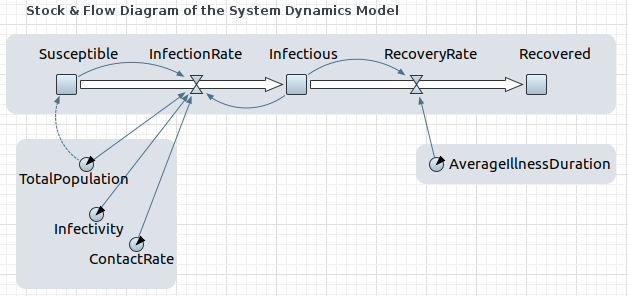
\includegraphics[width=.5\textwidth, angle=0]{./fig/SIR_SD_STOCKFLOW_DIAGRAMM.png}
	\caption{Visual System Dynamics Diagram of the SIR model in AnyLogic Personal Learning Edition 8.3.1.}
	\label{fig:sir_stockflow_diagram}
\end{figure}

Still, implementing System Dynamics directly in code is not as straight forward and involves numerical integration which can be quite tricky to get right. Thus, the aim of this paper is to look into how System Dynamics models can be implemented in code correctly without the use of a simulation package. We use the well known SIR model \cite{kermack_contribution_1927} from epidemiology to demonstrate our approach.

Our language of choice is Haskell because it emphasises a declarative programming style in which one describes \textit{what} instead of \textit{how} to compute. Further it allows to rule out interference with non-deterministic influences or side-effects already at compile-time. This is of fundamental importance for System Dynamics because it behaves completely deterministic and involves no stochastics or non-determinism whatsoever. Also, we make use of Functional Reactive Programming which allows to express continuous-time systems in a functional way. 

We show that by this approach we can arrive at correct-by-construction implementations of System Dynamic models. This means that the correctness of the code is obvious because we have closed the gap between the model specification and its implementation. Thus, the contribution of the paper is the demonstration of how to implement correct-by-construction System Dynamics simulations using Haskell and Functional Reactive Programming.

\section{Testing / Verification}
TODO: explore ABS testing in pure functional Haskell
- we need to distinguish between two types of testing/verification
	-> 1. testing/verification of models for which we have real-world data or an analytical solution which can act as a ground-truth. examples for such models are the SIR model, stock-market simulations, social simulations of all kind
	-> 2. testing/verification of models which are just exploratory and which are only be inspired by real-world phenomena. examples for such models are Epsteins Sugarscape and Agent\_Zero
	
\subsection{Black Box Verification}
Defined as treating the functionality to test as a black box with inputs and outputs and comparing controlled inputs to expected outputs.

In Black Box Verification one generally feeds input and compares it to expected output. In the case of ABS we have two things to black-box test:
\begin{enumerate}
	\item Agent Behaviour - test isolated agent behaviour under given inputs using unit- and property-based testing
	\item Simulation Dynamics - compare emergent dynamics of the ABS as a whole under given inputs to an analytical solution / real-world dynamics in case there exists some using statistical tests
	\item Hypotheses- test whether hypotheses are valid / invalid using unit- and property-based testing. TODO: how can we formulate hypotheses in unit- and/or property-based tests?
\end{enumerate}

- testing of the final dynamics: how close do they match the analytical solution
- can we express model properties in tests e.g. quickcheck?
- property-testing shines here
- isolated tests: how easy can we test parts of an agent / simulation?

\subsubsection{Finding optimal $\Delta t$}
The selection of the right $\Delta t$ can be quite difficult in FRP because we have to make assumptions about the system a priori. One could just play it safe with a very conservatively selected small $\Delta t <= 0.1$ but the smaller $\Delta t$, the lower the performance as it quickly multiplies the number of steps to calculate. Obviously one wants to select the \textit{optimal} $\Delta t$, which in the case of ABS is the largest possible $\Delta t$ for which we still get the correct simulation dynamics.
To find out the \textit{optimal} $\Delta t$ one can make direct use of the Black Box tests: start with a large $\Delta t = 1.0$ and reduce it by half every time the tests fail until no more tests fail - if for $\Delta t = 1.0$ tests already pass, increasing it may be an option. It is important to note that although isolated agent behaviour tests might result in larger $\Delta t$, in the end when they are run in the aggregate system, one needs to sample the whole system with the smallest $\Delta t$ found amongst all tests. Another option would be to apply super-sampling to just the parts which need a very small $\Delta t$ but this is out of scope of this paper.

\subsubsection{Agents as signals}
Agents \textit{might} behave as signals in FRP which means that their behaviour is completely determined by the passing of time: they only change when time changes thus if they are a signal they should stay constant if time stays constant. This means that they should not change in case one is sampling the system with $\Delta t = 0$. Of course to prove whether this will \textit{always} be the case is strictly speaking impossible with a Black Box verification but we can gain a good level of confidence with them also because we are staying pure. It is only through white box verification that we can really guarantee and prove this property.

\subsubsection{Comparison of dynamics against existing data}
- utilise a statistical test with H0 "ABS and comparison is not the same" and H1 "ABS and comparison is the same"
- how many replications and how do we average?
- which statistical test do we implement? (steward robinson simulation book, chapter 12.4.4)
	-> Normalizsed Mean Squared Error (NMSE)
	-> TODO: implement confidence interval 
	-> TODO: what about chi-squared?
	-> TODO: what about paired-t confidence interval

IMPORTANT: this is not what we are after here in this paper, statistical tests are a science on their own and there actually exists quite a large amount of literature for conducting statistical tests on ABS dynamics: Robinson Book (TODO: find additional literature)	

\subsection{White Box Verification}
White-Box verification is necessary when we need to reason about properties like \textit{forever}, \textit{never}, which cannot be guaranteed from black-box tests. Additional help can be coverage tests with which we can show that all code paths have been covered in our tests.

\section{Verification of SIR}
In this section we verify our agent-based implementation of the SIR model. Verification of our implementation should be fairly straight-forward and easy as the model is given in differential equations which gives us a formal specification of the model which we can use directly in our verification process. We will also conduct white-box verification and for one property it will be the only way of ensuring that our model is correct as we cannot guarantee it through black-box verification.

\subsection{Black Box Verification}
\subsubsection{Agent Behaviour}
When conducting black-box testing for the SIR model, we test if the \textit{isolated} behaviour of an agent in all three states Susceptible, Infected and Recovered, corresponds to model specifications. The crucial thing though is that we are dealing with a stochastic system where the agents act \textit{on averages}, which means we need to average our tests as well.

The interface of the agent behaviours are defined below. When running the SF with a given $\Delta t$ one has to feed in the state of all the other agents as input and the agent outputs its state it is after this $\Delta t$.

\begin{minted}{haskell}
data SIRState 
  = Susceptible 
  | Infected 
  | Recovered
  
type SIRAgent = SF [SIRState] SIRState

susceptibleAgent :: RandomGen g => g -> SIRAgent
infectedAgent :: RandomGen g => g -> SIRAgent
recoveredAgent :: SIRAgent
\end{minted}


\paragraph{Susceptible Behaviour}
A susceptible agent \textit{may} become infected, depending on the number of infected agents in relation to non-infected the susceptible agent has contact to. To make this property testable we run a susceptible agent for 1.0 time-unit (note that we are sampling the system with small $\Delta t$ e.g. 0.1) and then check if it is infected - that is it returns infected as its current state. Obviously we need to pay attention to the fact that we are dealing with a stochastic system thus we can only talk about averages and thus it does not suffice to only run a single agent but we are repeating this for e.g. $N = 10.000$ agents (all with different RNGs). We then need a formula for the required fraction of the N agents which should have become infected on average. Per 1.0 time-unit, a susceptible agent makes \textit{on average} contact with $\beta$ other agents where in the case of a contact with an infected agent the susceptible agent becomes infected with a given probability $\gamma$. In this description there is another probability hidden, which is the probability of making contact with an infected agent which is simply the ratio of number of infected agents to number not infected agents. The formula for the target fraction of agents which become infected is then: $\beta * \gamma * \frac{number of infected}{number of non-infected}$. To check whether this test has passed we compare the required amount of agents which on average should become infected to the one from our tests (simply count the agents which got infected and divide by N) and if the value lies within some small $\epsilon$ then we accept the test as passed.

Obviously the input to the susceptible agents which we can vary is the set of agents with which the susceptible agents make contact with. To save us from constructing all possible edge-cases and combinations and testing them with unit-tests we use QuickCheck which creates them randomly for us and reduces them also to all relevant edge-cases. This is an example for how to use property-based testing in ABS where QuickCheck can be of immense help generating random test-data to cover all cases.

TODO: derive the target-fraction formula from the differential equations
TODO: can we encode this somehow on a type level using dependent types? then we don't need to test this property any more

\paragraph{Infected Behaviour}
An infected agent \textit{will always} recover after a finite time, which is \textit{on average} after $\delta$ time-units. Note that this property involves stochastics too, so to test this property we run a large number of infected agents e.g. $N = 10.000$ (all with different RNGs) until they recover, record the time of each agents recovery and then average over all recovery times. To check whether this test has passed we compare the average recovery times to $\delta$ and if they lie within some small $\epsilon$ then we accept the test as passed.
We use QuickCheck in this case as well to generate the set of other agents as input for the infected agents. Strictly speaking this would not be necessary as an infected agent never makes contact with other agents and simply ignores them - we could as well just feed in an empty list. We opted for using QuickCheck for the following reasons:

\begin{itemize}
	\item We wanted to stick to the interface specification of the agent-implementation as close as possible which asks to pass the states of all agents as input.
	\item We shouldn't make any assumptions about the actual implementation and if it REALLY ignores the other agents, so we strictly stick to the interface which requires us to input the states of all the other agents.
	\item The set of other agents is ignored when determining whether the test has failed or not which indicates by construction that the behaviour of an infected agent does not depend on other agents.
	\item We are not just running a single replication over 10.000 agents but 100 of them which should give black-box verification more strength.
\end{itemize}

TODO: derive the average formula from the differential equations
TODO: can we encode this somehow on a type level using dependent types? then we don't need to test this property any more

\paragraph{Recovered Behaviour}
A recovered agent will stay in the recovered state \textit{forever}. Obviously we cannot write a black-box test that truly verifies that because it had to run in fact forever. In this case we need to resort to White Box Verification (see below).

Because we use multiple replications in combination with QuickCheck obviously results in longer test-runs (about 5 minutes on my machine)
In our implementation we utilized the FRP paradigm. It seems that functional programming and FRP allow extremely easy testing of individual agent behaviour because FP and FRP compose extremely well which in turn means that there are no global dependencies as e.g. in OOP where we have to be very careful to clean up the system after each test - this is not an issue at all in our \textit{pure} approach to ABS.

\subsubsection{Simulation Dynamics}
We won't go into the details of comparing the dynamics of an ABS to an analytical solution, that has been done already by \cite{macal_agent-based_2010}. What is important is to note that population-size matters: different population-size results in slightly different dynamics in SD => need same population size in ABS (probably...?). Note that it is utterly difficult to compare the dynamics of an ABS to the one of a SD approach as ABS dynamics are stochastic which explore a much wider spectrum of dynamics e.g. it could be the case, that the infected agent recovers without having infected any other agent, which would lead to an extreme mismatch to the SD approach but is absolutely a valid dynamic in the case of an ABS. The question is then rather if and how far those two are \textit{really} comparable as it seems that the ABS is a more powerful system which presents many more paths through the dynamics.
TODO: i really want to solve this for the SIR approach
	-> confidence intervals?
	-> NMSE?
	-> does it even make sense?

\subsubsection{Finding optimal $\Delta t$}
Obviously the \textit{optimal} $\Delta t$ of the SIR model depends heavily on the model parameters: contact rate $\beta$ and illness duration $\delta$. We fixed them in our tests to be $\beta = 5$ and $\delta = 15$. By using the isolated behaviour tests we found an optimal $\Delta t = 0.125$ for the susceptible behaviour and $\Delta t = 0.25$ for the infected behaviour. TODO: dynamics comparison?

\subsubsection{Agents as signals}
Our SIR agents \textit{are} signals due to the underlying continuous nature of the analytical SIR model and to some extent we can guarantee this through black box testing. For this we write tests for each individual behaviour as previously but instead of checking whether agents got infected or have recovered we assume that they stay constant: they will output always the same state when sampling the system with $\Delta t = 0$. The tests are conceptual the complementary tests of the previous behaviour tests so in conjunction with them we can assume to some extent that agents are signals. To prove it, we need to look into white box verification as we cannot make guarantees about properties which should hold \textit{forever} in a computational setting.

\subsection{White Box Verification}
In the case of the SIR model we have the following invariants: 
\begin{itemize}
	\item A susceptible agent will \textit{never} make the transition to recovered.
	\item An infected agent will \textit{never} make the transition to susceptible.
	\item A recovered agent will \textit{forever} stay recovered.
\end{itemize}

All these invariants can be guaranteed when reasoning about the code. An additional help will be then coverage testing with which we can show that an infected agent never returns susceptible, and a susceptible agent never returned infected given all of their functionality was covered which has to imply that it can never occur!

Lets start with looking at the recovered behaviour as it is the simplest one. We then continue with the infected behaviour and end with the susceptible behaviour as it is the most complex one.

\paragraph{Recovered Behaviour}
The implementation of the recovered behaviour is as follows:

\begin{minted}{haskell}
recoveredAgent :: SIRAgent
recoveredAgent = arr (const Recovered)
\end{minted}

Just by looking at the type we can guarantee the following:
\begin{itemize}
	\item it is pure, no side-effects of any kind can occur
	\item no stochasticity possible because no RNG is fed in / we don't run in the random monad
\end{itemize}

The implementation is as concise as it can get and we can reason that it is indeed a correct implementation of the recovered specification: we lift the constant function which returns the Recovered state into an arrow. Per definition and by looking at the implementation, the constant function ignores its input and returns always the same value. This is exactly the behaviour which we need for the recovered agent. Thus we can reason that the recovered agent will return Recovered \textit{forever} which means our implementation is indeed correct.

\paragraph{Infected Behaviour}
\begin{minted}{haskell}
infectedAgent :: RandomGen g 
              => g 
              -> Double
              -> SIRAgent
infectedAgent g illnessDuration = 
    switch 
      infected 
      (const recoveredAgent)
  where
    infected :: SF [SIRState] (SIRState, Event ())
    infected = proc _ -> do
      recEvt <- occasionally g illnessDuration () -< ()
      let a = event Infected (const Recovered) recEvt
      returnA -< (a, recEvt)
\end{minted}

By looking at the types we can reason that there \textit{may} be some stochasticity involved (the function may choose to ignore the RNG) and that we are again pure. TODO: not finished yet

\paragraph{Susceptible Behaviour}
\begin{minted}{haskell}
susceptibleAgent :: RandomGen g 
                 => g 
                 -> Double
                 -> Double
                 -> Double 
                 -> SIRAgent
susceptibleAgent g contactRate infectivity illnessDuration = 
    switch
      (susceptible g) 
      (const (infectedAgent g illnessDuration))
  where
    susceptible :: RandomGen g => g -> SF [SIRState] (SIRState, Event ())
    susceptible g = proc as -> do
      makeContact <- occasionally g (1 / contactRate) () -< ()

      -- NOTE: strangely if we are not splitting all if-then-else into
      -- separate but only a single one, then it seems not to work,
      -- dunno why
      if isEvent makeContact
        then (do
          a <- drawRandomElemSF g -< as
          case a of
            Just Infected -> do
              i <- randomBoolSF g infectivity -< ()
              if i
                then returnA -< (Infected, Event ())
                else returnA -< (Susceptible, NoEvent)
            _       -> returnA -< (Susceptible, NoEvent))
        else returnA -< (Susceptible, NoEvent)
\end{minted}


\section{Verification of Sugarscape}
Sugarscape is an exploratory model inspired by real-world phenomenon which means it has lots of hypotheses implicit in the model but there does not exist real-world data / dynamics against which one could validate the simulated dynamics. Still we can conduct black-box verification because we have an informal model specification but we cannot do any statistical testing of simulated dynamics as we don't have data acting as ground-truth. But what we can do and what we will explore extensively in this section is how we can encode hypotheses about the dynamics (prior to running the simulation) in unit- and property-based tests and check them. Obviously white-box verification applies as well because we can reason about the code whether it matches the informal model specification or not.

\subsection{Black Box Verification}
\subsubsection{Agent Behaviour}

\subsubsection{Hypotheses}

\subsection{White Box Verification}


\section{Dependent Types in Agent-Based Simulation}

The strong static type system of Haskell allows us to guarantee a lot already at compile time:
\begin{itemize}
	\item Purity - no side-effects possible at all 
	\item Monad - controlled, explicit side-effects possible
	\item generic types allow to guarantee for all
\end{itemize}

Dependent Types in Idris bring the strong static type system of Haskell to a new level, which allows us to both guarantee more things at compile time and express things through type-level computations. This means the following at compile time

\begin{itemize}
	\item Ruling out ever larger classes of bugs
	\item Dependent State Machines
	\item Dependent Agent Interactions
	\item Flow Of Time
	\item Totality
	\item Constructive Proofs
\end{itemize}

\subsection{Ruling out Bugs}
\begin{enumerate}
	\item Index out of bounds access of Lists and Vectors can be guaranteed not to happen any more when using proofs of existence of the element in the list or vector.
	\item Size of list or vector stays constant / increases / decreases / sum of length of multiple vectors guaranteed to be of some number
\end{enumerate}

The question is how far we can generalise our approaches because we fear that the downside of using dependently typed abs is that every implementation needs to start from Scratch: we cant write a general library for it like chimera because the more we put into types, the more specific it is => individual implementation which reuses existing 'patterns' like state machines, messages,...

\subsection{Dependent State Machines}
dependent state machines in abs for internal state because that is very Common in ABS

\subsection{Dependent Agent Interactions}
\subsubsection{Agent Transactions}
dependently typed message protocols in ABS because its very common, and easily done thorugh methods in OOP: sugarscape mating and trading protocol
\subsubsection{Data Flow}
TODO: can dependent types be used in the Data Flow Mechanism?
\subsubsection{Event Scheduling}
TODO: can dependent types be used in the event-scheduling mechanism?

\subsection{Flow Of Time}
TODO: can dependent types be used to express the flow of time and its strongly monotonic increasing?

\subsection{Totality}
totality of parts or the whole simulation

\subsection{Constructive Proofs}
- An agent-based model and the simulated dynamics of it is itself a constructive proof which explain a real-world phenomenon sufficiently good
- proof of the existence of an agent: holds always only for the current time-step

\section{Towards Dependently Typed Verification}
Independent of the programming paradigm, there exist fundamentally two approaches implementing agent-based simulation: time- and event-driven. In the time-driven approach, the simulation is stepped in fixed $\Delta t$ and all agents are executed at each time-step - they act virtually in lock-step at the same time. The approach is inspired by the theory of continuous system dynamics (TODO: cite).
In the event-driven approach, the system is advanced through events, generated by the agents, and the global system state changes by jumping from event to event, where the state is held constant in between. The approach is inspired by discrete event simulation (DES) (TODO: citation) which is formalized in the DEVS formalism \cite{zeigler_theory_2000}.

In a preceding paper we investigated how to derive a time-driven pure functional ABS approach in Haskell (TODO: cite my paper). We came to quite satisfactory results and implemented also a number of agent-based models of various complexity (TODO: cite schelling, sugarscape, agent zero). Still we identified weaknesses due to the underlying functional reactive programming (FRP) approach. It is possible to define partial implementations which diverge during runtime, which may be difficult to determine for complex models for a programmer at compile time. Also sampling the system with fixed $\Delta t$ can lead to severe performance problems when small $\Delta t$ are required, as was shown in our paper. The later problem is well known in the simulation community and thus as a remedy an event-driven approach was suggested \cite{meyer_event-driven_2014}.
In this paper for the first time, we derive a pure functional event-driven agent-based simulation. Instead of using Haskell, which provides already libraries for DES \cite{sorokin_aivika_2015}, we focus on the dependently typed pure functional programming language Idris. In our previous paper we hypothesised that dependent types may offer interesting new insights and approaches to ABS but it was unclear how exactly we can make use of them, which was left for further research. In this paper we hypothesise that, as opposed to a time-driven approach, the even-driven approach is especially suited to make proper use of dependent types due to its different nature. Note that both a pure functional event-driven approach to ABS \textit{and} the use of dependent types in ABS has so far never been investigated, which is the unique contribution of this paper.
If we can construct a dependently typed program of the SIR ABM which is total, then we have a proof-by-construction that the SIR model reaches a steady-state after finite time

Dependent Types are the holy grail in functional programming as they allow to express even stronger guarantees about the correctness of programs and go as far where programs and types become constructive proofs \cite{wadler_propositions_2015} which must be total by definition \cite{thompson_type_1991}, \cite{altenkirch_why_2005}, \cite{altenkirch_pi_sigma:_2010}, \cite{program_homotopy_2013}. Thus the next obvious step is to apply them to our pure functional approach of agent-based simulation. So far no research in applying dependent types to agent-based simulation exists at all and it is not clear whether dependent types do make sense in this setting. We explore this for the first time and ask more specifically how we can add dependent types to our pure functional approach, which conceptual implications this has for ABS and what we gain from doing so. Note that we can only scratch the surface and lay down basic ideas and leave a proper in-depth treatment of this topic for further research. We use Idris \cite{brady_idris_2013}, \cite{brady_type-driven_2017} as language of choice as it is very close to Haskell with focus on real-world application and running programs as opposed to other languages with dependent types e.g. Agda and Coq which serve primarily as proof assistants.

Dependent Types promise the following:

\begin{enumerate}
	\item Types as proofs - In dependently types languages, types can depend on any values and are first-class objects themselves. TODO: make more clear

	\item Totality and termination - Constructive proofs must terminate, this means a well-typed program (which is itself a proof) is always terminating which in turn means that it must consist out of total functions. A total function is defined by \cite{brady_type-driven_2017} as: it terminates with a well-typed result or produces a non-empty finite prefix of a well-typed infinite result in finite time. Idris is turing complete but is able to check the totality of a function under some circumstances but not in general as it would imply that it can solve the halting problem. Other dependently typed languages like Agda or Coq restrict recursion to ensure totality of all their functions - this makes them non turing complete.
\end{enumerate}

%An agent can be seen as a potentially infinite stream of continuations which at some point could return information to stop evaluating the next item of the stream which allows an agent to terminate.
%correspondence between temporal logics and FRP due to jeffery: is abs just another temporal logic?

%Ionesus talk on dependently typed programming in scientific computing
%https://www.pik-potsdam.de/members/ionescu/cezar-ifl2012-slides.pdf
%Ionescus talk on Increasingly Correct Scientific Computing
%https://www.cicm-conference.org/2012/slides/CezarIonescu.pdf
%Ionescus talk on Economic Equilibria in Type Theory
%https://www.pik-potsdam.de/members/ionescu/cezar-types11-slides.pdf
%Ionescus talk on Dependently-Typed Programming in Economic Modelling
%https://www.pik-potsdam.de/members/ionescu/ee-tt.pdf

dependent-types:
-> encode model-invariants on a meta-level
-> encode dynamics (what? feedbacks? positive/negative) on a meta-level
-> totality equals steady-state of a simulation, can enforce totality if required through type-level programming
-> probabilistic types can encode probability distributions in types already about which we can then reason
-> can we encode objectives in types?

\subsection{Dependently Typed SIR}
Intuitively, based upon our model and the equations we can argue that the SIR model enters a steady state as soon as there are no more infected agents. Thus we can informally argue that a SIR model must always terminate as:
\begin{enumerate}
	\item Only infected agents can infect susceptible agents.
	\item Eventually after a finite time every infected agent will recover.
	\item There is no way to move from the consuming \textit{recovered} state back into the \textit{infected} state \footnote{There exists an extended SIR model, called SIRS which adds a cycle to the state-machine by introducing a transition from recovered to susceptible but we don't consider that here.}.
\end{enumerate}

Thus a SIR model must enter a steady state after finite steps / in finite time. 

This result gives us the confidence, that the agent-based approach will terminate, given it is really a correct implementation of the SD model. Still this does not proof that the agent-based approach itself will terminate and so far no proof of the totality of it was given. Dependent Types and Idris ability for totality and termination checking should theoretically allow us to proof that an agent-based SIR implementation terminates after finite time: if an implementation of the agent-based SIR model in Idris is total it is a proof by construction. Note that such an implementation should not run for a limited virtual time but run unrestricted of the time and the simulation should terminate as soon as there are no more infected agents. We hypothesize that it should be possible due to the nature of the state transitions where there are no cycles and that all infected agents will eventually reach the recovered state. 
Abandoning the FRP approach and starting fresh, the question is how we implement a \textit{total} agent-based SIR model in Idris. Note that in the SIR model an agent is in the end just a state-machine thus the model consists of communicating / interacting state-machines. In the book \cite{brady_type-driven_2017} the author discusses using dependent types for implementing type-safe state-machines, so we investigate if and how we can apply this to our model. We face the following questions: how can we be total? can we even be total when drawing random-numbers? Also a fundamental question we need to solve then is how we represent time: can we get both the time-semantics of the FRP approach of Haskell AND the type-dependent expressivity or will there be a trade-off between the two?

-- TODO: express in the types
-- SUSCEPTIBLE: MAY become infected when making contact with another agent
-- INFECTED:    WILL recover after a finite number of time-steps
-- RECOVERED:   STAYS recovered all the time

-- SIMULATION:  advanced in steps, time represented as Nat, as real numbers are not constructive and we want to be total
--              terminates when there are no more INFECTED agents



%A susceptible agent can only become infected when it comes into contact with an infected agent. The probability of a susceptible agent making contact with an infected one is naturally (number of infected agents) / (total number of agents). For the infection to occur we multiply the contact with the infectivity parameter \Gamma. A susceptible agent makes on average \Beta contacts per time-unit. This results in the following formula:
%
%\begin{align}
%prob &= \frac{I \beta \gamma}{N} \\
%\end{align}
%
%This is for a single agent, which we then need to multiply by the number of susceptible agents because all of them make contact.
%
%TODO: implement sir with state-machine approach from Idris. an idea would be to let infected agents generate infection- actions: the more infected agents the more infection-actions => zero infected agents mean zero infection actions. this list can then be reduced?
%
%can we also emulate SD in Idris and formulate positive/negative feedback loops in types?

% Bibliography
%\bibliographystyle{../../../templates/IEEEtran/bibtex/IEEEtran}
\bibliographystyle{../../templates/acmart/ACM-Reference-Format}
\bibliography{../../../references/phdReferences.bib}

\end{document}